\section{Kalman Filter for prediction}

Let's examine a straightforward system devoid of external influences, characterized by linearity and time-invariance.

\subsection{System description}
We're dealing with a multiple input multiple output system denoted as $\mathcal{S}$, described by the following equations:
\[\mathcal{S}:\begin{cases}
    x(t+1)=Fx(t)+Gu(t)+v_1(t) \\
    y(t)=Hx(t)+Du(t)+v_2(t)
\end{cases}\]
Here: 
\[x(t)=\begin{bmatrix} x_1(t) \\ x_2(t) \\ \vdots \\ x_n(t) \end{bmatrix} \quad u(t)=\begin{bmatrix} u_1(t) \\ u_2(t) \\ \vdots \\ u_m(t) \end{bmatrix} \quad y(t)=\begin{bmatrix} y_1(t) \\ y_2(t) \\ \vdots \\ y_p(t) \end{bmatrix}\]
In this configuration, there are $n$ states, $p$ inputs, and $m$ outputs. 

\paragraph*{First White Noise}
The vector White Noise $v_1(t)$ characterizes internal disturbances and minor model inaccuracies, with zero mean and variance $V_1$:
\[v_1(t)=\begin{bmatrix} v_{11}(t) \\ v_{12}(t) \\ \vdots \\ v_{1n}(t) \end{bmatrix}\]
It's termed model noise. 
Its properties are:
\begin{enumerate}
    \item Each element of the $v_1(t)$ matrix has an expected value of zero:
        \[\mathbb{E}\left[v_1(t)\right]=0\]
    \item The covariance matrix of $v_1(t)$ is determined as:
        \[V_1=\mathbb{E}\left[v_1(t)v_1(t)^T\right]\]
        This matrix is square, symmetric, and positive semi-definite.
    \item Covariance is zero:
        \[\mathbb{E}\left[v_1(t)v_1(t-\tau)^T\right]=0\qquad \forall t, \forall\tau\neq 0\]
\end{enumerate}

\paragraph*{Second White Noise}
The vector White Noise $v_2(t)$ characterizes internal disturbances and minor model inaccuracies, with zero mean and variance $V_2$:
\[v_2(t)=\begin{bmatrix} v_{21}(t) \\ v_{22}(t) \\ \vdots \\ v_{2p}(t) \end{bmatrix}\]
It's termed sensor noise. 
Its properties are:
\begin{enumerate}
    \item Each element of the $v_2(t)$ matrix has an expected value of zero:
        \[\mathbb{E}\left[v_2(t)\right]=0\]
    \item The covariance matrix of $v_2(t)$ is determined as:
        \[V_2=\mathbb{E}\left[v_2(t)v_2(t)^T\right]\]
        This matrix is square, symmetric, and assumed to be positive definite, a requirement for applications involving the Differential Riccati Equation.
    \item Covariance is zero:
        \[\mathbb{E}\left[v_2(t)v_2(t-\tau)^T\right]=0\qquad \forall t, \forall\tau\neq 0\]
\end{enumerate}

\paragraph*{Assumptions}
Given the dynamical nature of the system, certain assumptions about initial conditions are necessary. 
We assume that:
\begin{itemize}
    \item The expected value of the initial state $x(1)$ is $x_0$: 
        \[\mathbb{E}\left[x(1)\right]=x_0\]
    \item The expected value of the outer product of the difference between the initial state and $x_0$ with its transpose is $P_0$, where $P_0$ is non-negative: 
        \[\mathbb{E}\left[\left(x(1)-x_0\right)\left(x(1)-x_0^T\right)\right]=P_0\geq 0\]
\end{itemize}
This approach provides a probabilistic description of the initial state, encompassing both its mean value and variance.
If $P_0=0$, it implies precise knowledge of the initial state.

\paragraph*{Correlation between the two White Noises}
We make the assumption that the correlation between $v_1(t)$ and $v_2(t-\tau)$ is given by:
\[\mathbb{E}=\left[v_1(t)v_2(t-\tau)^T\right]=\begin{cases}
    0 \qquad\quad\text{if }\tau\neq 0 \\
    V_{12} \qquad\:\text{if }\tau= 0
\end{cases}\]
Typically, $V_{12}=0$.

\paragraph*{Correlation between the White Noises and the initial state}
It's assumed that both White Noises $v_1(t)$ and $v_2(t)$ are uncorrelated with the initial state $x(1)$. 
This technical assumption ensures the theoretical optimality of the Kalman Filter.

\subsection{One step predictor}
We utilize the following solution:
\[\begin{cases}
    \hat{x}(t+1|t)=F\hat{x}(t|t-1)+K(t)e(t) \\ 
    \hat{y}(t+1|t)=H\hat{x}(t|t-1) \\
    e(t)=y(t)-\hat{y}(t|t-1) \\
    K(t)=\left(FP(t)H^T+V_{12}\right)\left(FP(t)H^T+V_2\right)^{-1} \\
    P(t+1)=\left(FP(T)F^T+V_1\right)-\left(FP(t)H^T+V_{12}\right)\left(HP(t)H^T+V_{2}\right)^{-1}\left(FP(t)H^T+V_{12}\right)^T
\end{cases}\]
Each equation serves a distinct purpose:
\begin{enumerate}
    \item \textit{State equation}: predicts the next state based on the current state and the system's dynamics.
    \item \textit{Output equation}: predicts the next output based on the predicted state.
    \item \textit{Error equation}: computes the prediction error between the actual output and the predicted output.
    \item \textit{Gain equation}: computes the optimal Kalman gain.
    \item \textit{Differential Riccati Equation}: computes the covariance matrix of the one-step prediction error of the states.
\end{enumerate}
To ensure the solution's validity, we require initial conditions:
\[\begin{cases}
    \hat{x}(1|0)=x_0 \\
    P(1)=P_0
\end{cases}\]

\paragraph*{Differential Riccati Equation and gain structure}
The structure of $K(t)$ and the Differential Riccati Equation  is block-wise. 
The three essential blocks involved are:
\begin{itemize}
    \item State block: $FP(T)F^T+V_1$.
    \item Output block: $HP(t)H^T+V_{2}$.
    \item Mix block: $FP(t)H^T+V_{12}$.
\end{itemize}

\paragraph*{Differential Riccati Equation}
The Differential Riccati Equation a specialized type of nonlinear matrix difference equation. 
It represents an autonomous system devoid of inputs:
\[\begin{cases}
    P(t+1)=f(P(t)) \\
    P(1)=P_0
\end{cases}\]
To ensure the existence of the Differential Riccati Equation at all time instants, $HP(t)H^T+V_2$ must be invertible. 
Given our assumption that $V_2$ is positive semi-definite, the full matrix becomes positive definite and thus invertible.

\paragraph*{Prediction error}
$P(t)$ is a symmetric $n \times n$  matrix representing the covariance matrix of the one-step prediction error of the states:
\[P(t)=\mathbb{E}\left[\left(x(t)-\hat{x(t|t-1)}\right)\left(x(t)-\hat{x(t|t-1)}\right)^T\right]=\text{Var}\left[x(t)-\hat{x(t|t-1)}\right]\]

\paragraph*{Graphical representation}
The block diagram of the system and the Kalman Filter is depicted below:
\begin{figure}[H]
    \centering
    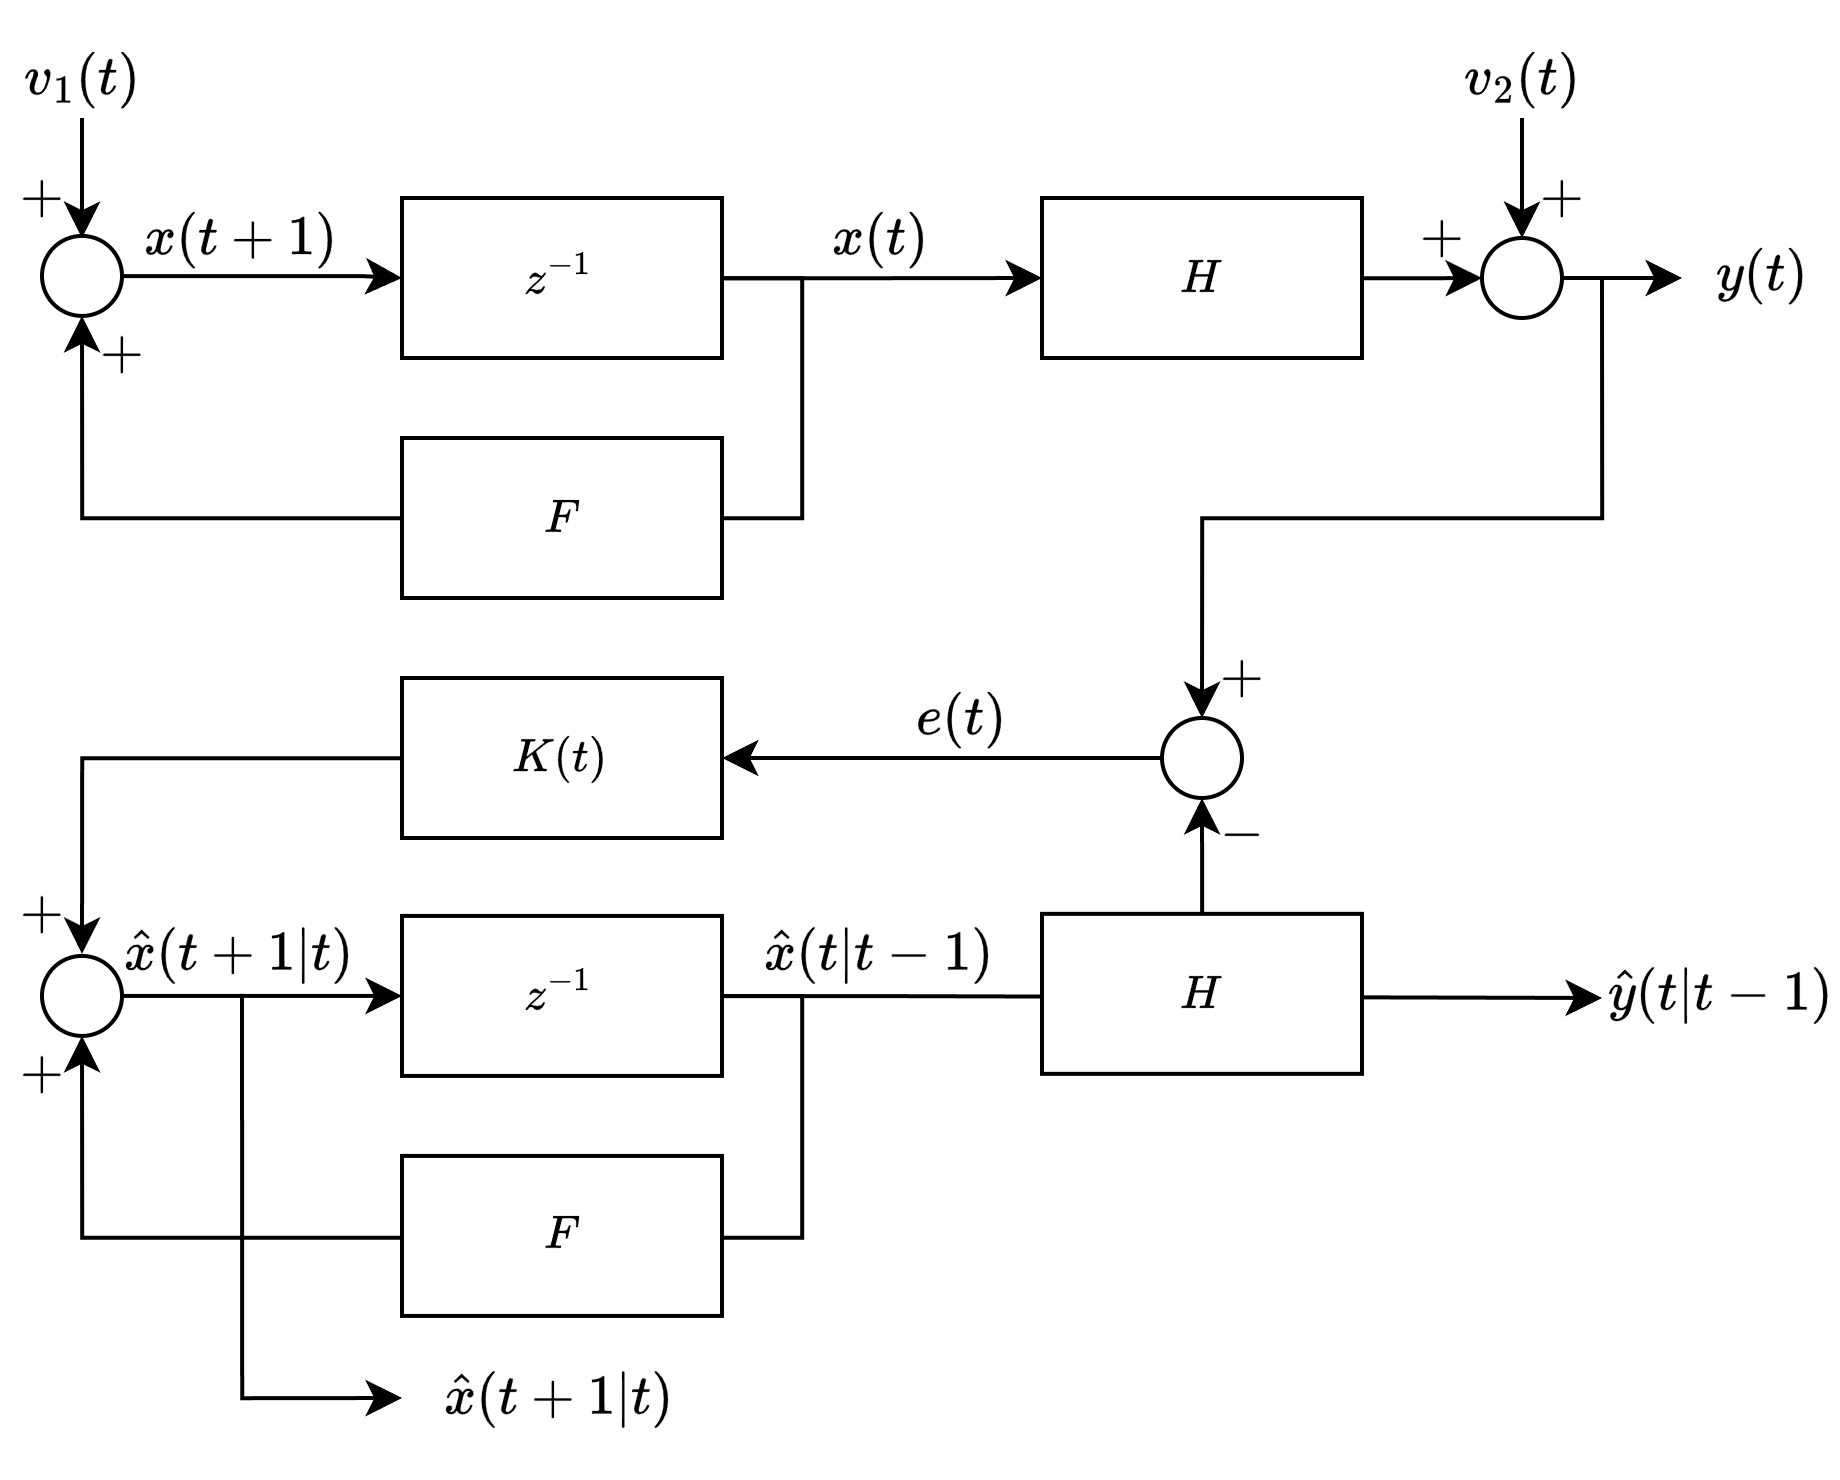
\includegraphics[width=0.75\linewidth]{images/kalman.png}
\end{figure}
The structure of the Kalman Filter is straightforward and intuitive:
\begin{itemize}
    \item It mimics the system's structure, excluding the two unmeasurable noises.
    \item It computes the real output and the estimated output, generating the output error:
        \[e(t)=y(t)-\hat{y}(t|t-1)\]
    \item It corrects the state equation in a feedback loop using a given $K(t)$ applied on $e(t)$. 
\end{itemize}
In essence, the Kalman Filter aims to track the real system with a feedback correction based on the output error. 
This concept, known as a state observer, predates Kalman. 
Kalman's contribution lies in providing the formula for the optimal correction gain $K(t)$. 

The optimal gain $K(t)$ plays a crucial role:
\begin{itemize}
    \item If $K(t)$ is too small, it underutilizes the information in $e(t)$. 
    \item If $K(t)$ is too large, it amplifies noises excessively, potentially leading to instability.
\end{itemize}
Since $K(t)$ is an $n \times p$ matrix, empirical tuning becomes impractical.